This chapter outlines the requirement specification of the system. This section describes the requirement analysis process. The process of gathering the requirements was done in collaboration with Tromsø IL.

\section{Overview}

The requirements evolved during the process of developing the system. Initially a requirement specification was designed from our perspective. We looked at the different analyze systems out there and what was in use at Alfheim today. Rather than going very wide providing all kind of analyses and statistics we narrowed it down to a very concrete system. A system that tries to to for many things may fell between two chairs, and at the end of the day not providing anything. You spend less time on each feature as you have more features thus reducing the quality on each feature.

The imagined system shall give you the key players in the offensive play of a given opponent soccer team. You shall be able to search on teams and individual players. Additionally you shall be able to see which areas of the pitch players are creating goal chances from. The system also needs a way of capturing data. This shall be an interface that enables you to store successful attacks for any match.

\begin{figure}[ht!]
\centering
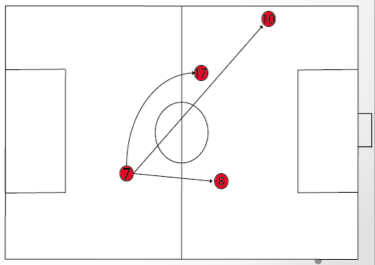
\includegraphics[width=50mm]{images/general/illustration_after_search2.png}
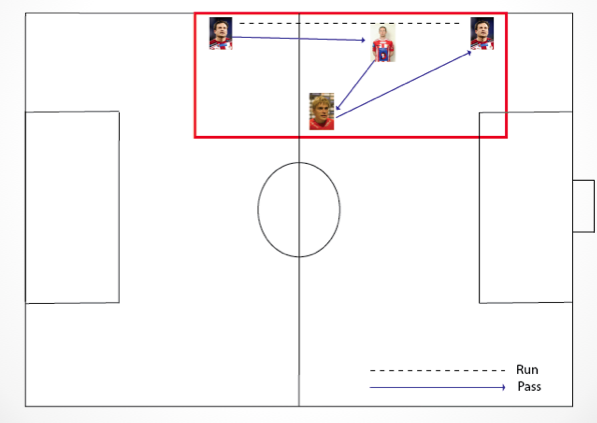
\includegraphics[width=50mm]{images/general/illustration_after_search.png}
\caption{Visioned illustration displaying key players and how they combine given you have queried on a team}
\label{overflow}
\end{figure}

\section{Capture}

A domain model for the captured data is crucial to set as early as possible in the process.  Changes to the model slows the development process. Captured data has to be re-captured and previous queries on data may fail due to missing fields. The domain model should reflect what we want to get out of the system. It sets the boundary's for which information we can pull from the system afterwards. When defining requirements Tromsø IL gave us a domain model they have used for a previous analytic project. It presented a analytic breakdown of all goals for Manchester United in the 2011/2012 season in Barclays Premier League. This domain model was used became our foundation for our domain model.

\begin{figure}[ht!]
\centering
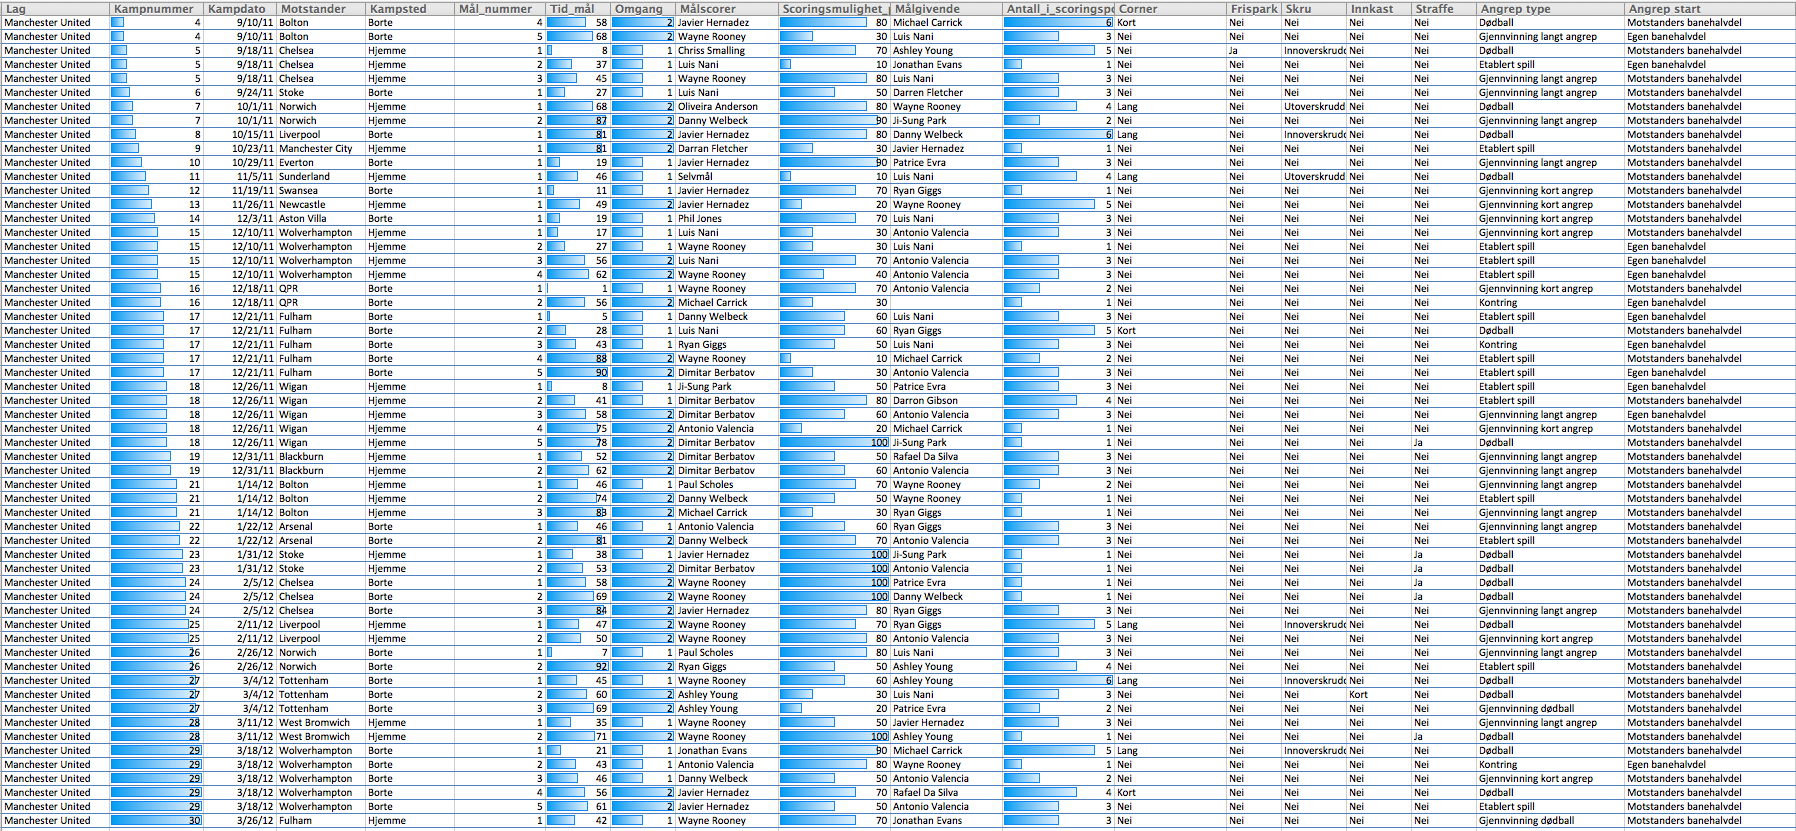
\includegraphics[width=50mm]{images/general/prev_domain_model.png}
\caption{A screencapture showing some data Tromsø IL captured in a previous analytic project}
\label{overflow}
\end{figure}

The visioned system need a datastore. The data should be stored in database that has a rich query language. This for being able to support the large range of queries on the data. Good support for aggregate functions is crucial.  The data will consist of text and integers.

Additionally a interface for input will be required. This interface should ensure that the input data is correct. For example when defining what type of attack the attack is, only the predefined options should be valid as input. 

Initially we wanted to build a database of all the matches in the Norwegian premier league. From each match every successful attack a team makes should be captured. From the attack started you registrate where the attack started, every pass including from/to co-ordinates, and what type of attack the attack can be categorized as. At last if there is a breaking point in the attack this should be captured. The breaking point of the attack is stored with a breakthrough player and what type of breakthrough it was.


\begin{figure}[ht!]
\centering
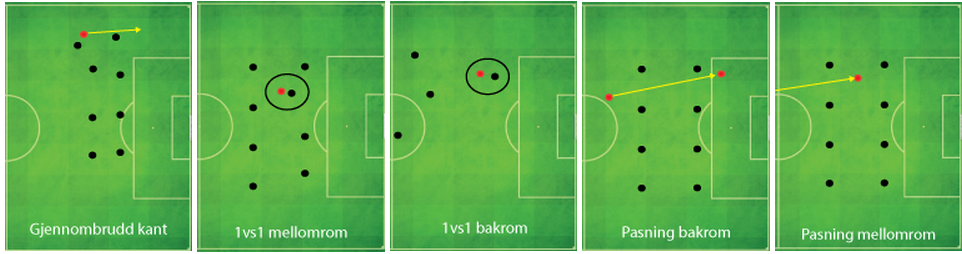
\includegraphics[width=50mm]{images/general/different_breakthroughs.png}
\caption{Illustrations of different breakthroughs we want to registrate}
\label{overflow}
\end{figure}

A definition of what a breakthrough player is: A player that does something extra that unbalance the other team. This can be a dribble past 1-2 players or a genius pass that opens deference of the opponents team. 

First problem was how to divide the pitch into zones. As we are looking for which zones the breaking point of the attack this is crucial for the searches on the data captured later on. During the development of the system several types of dividing was presented to the coaching staff. 

\begin{figure}[ht!]
\centering
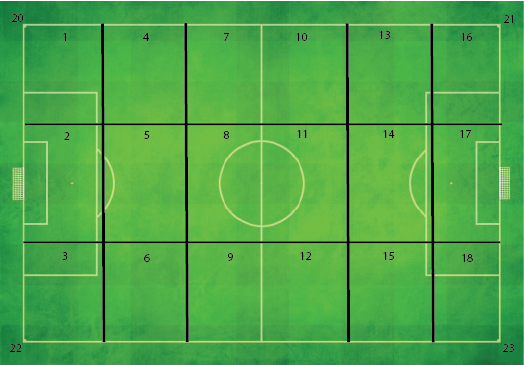
\includegraphics[width=100mm]{images/general/first_zones.png}
\caption{Dividing of pitch - the first suggestion had 18 zones}
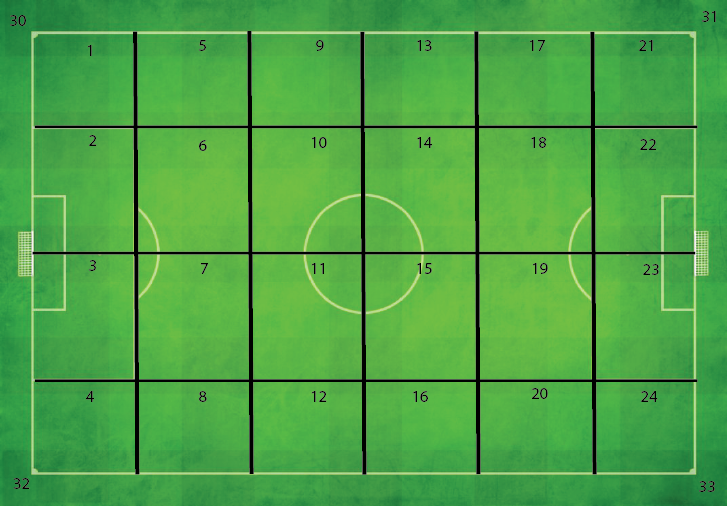
\includegraphics[width=100mm]{images/general/second_zones.png}
\caption{Dividing of pitch - the second suggestion had 24 zones}
\label{overflow}
\end{figure}

\section{Present}

The presentation of the data is a important aspect of the system. This will be where the end-users will spend their time. The presentation of data needs to be as simple as possible to understand. The coaching staff is no technical experts. The system is  aimed for them to use. Therefor the system will need to present statistics and other valuable information in clean and understandable way. In the end it is the 11 players the coach selects that performs all the actions, but the coach sets the style of play boundary's for players. The goal is to give the coach the opportunity to use the system, both analytic illustrations and statistics provided in the system, so he can better reach out to his players with his ideas. The better a coach can sell his ideas to the players the more they will believe in the philosophy, style of play and follow the game plan when out on the field.

We purpose a web interface here as it is accessible from many devices as long as you have a Internet connection and a up to date web browser. 


\Section{Summary}

\begin{figure}[ht!]
\centering
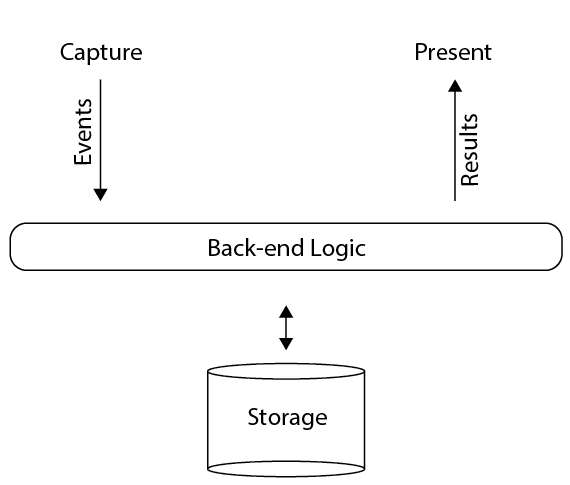
\includegraphics[width=150mm]{images/architecture/conceptual_architecture.png}
\caption{Conceptual arhitecture}
\label{overflow}
\end{figure}